\StartPlate{V11}{Three conductor columns are not interchangeable}{The scalar summand changes an epsilon exponent even when the ordinary conductor is unchanged.}
\begin{center}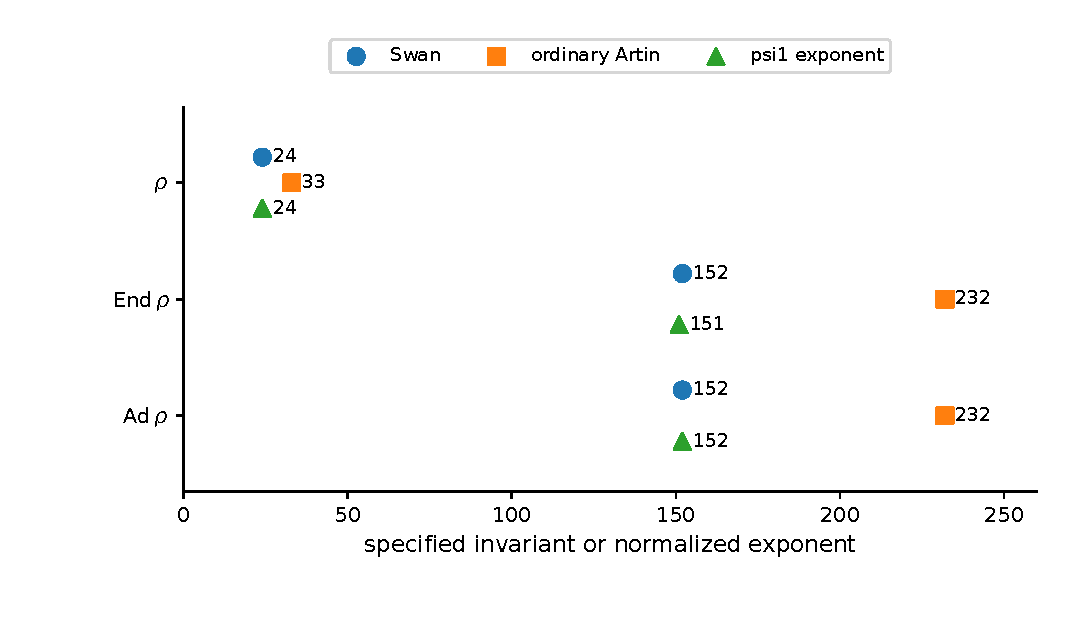
\includegraphics[width=\linewidth]{figures/V11.pdf}\end{center}
The ordinary conductor is $a(V)=\dim V-\dim V^{I_F}+\operatorname{Sw}(V)$. For the additive character $\psi_1$ trivial on $\mathfrak p_F$ but not on $\mathcal O_F$, the stated normalization gives $f_{\psi_1}(V)=a(V)-\dim V$.
\[
\begin{array}{c|rrr}
V&\operatorname{Sw}(V)&a(V)&f_{\psi_1}(V)\\
\rho&24&33&24\\
\operatorname{End}\rho&152&232&151\\
\operatorname{Ad}\rho&152&232&152
\end{array}
\]
Here $\operatorname{Ad}\rho$ means the trace-zero summand. The scalar summand in $\operatorname{End}\rho=\C\oplus\operatorname{Ad}\rho$ has zero ordinary conductor, but it contributes one to the dimension subtracted in the epsilon normalization.

The plot keeps the three definitions separate even when values happen to coincide. An exponent is still not the full epsilon factor. The arithmetic conductor inputs and additive-character convention are inherited from the audited progress paper, not freshly established by drawing these numbers.
\vfill\PlateSource{Exact normalization worksheet}{Part III, Section 22.1}{58}
